\documentclass{article}

% if you need to pass options to natbib, use, e.g.:
% \PassOptionsToPackage{numbers, compress}{natbib}
% before loading nips_2018

% ready for submission
% \usepackage{nips_2018}

% to compile a preprint version, e.g., for submission to arXiv, add
% add the [preprint] option:
% \usepackage[preprint]{nips_2018}

% to compile a camera-ready version, add the [final] option, e.g.:
\usepackage[final]{nips_2018}

% to avoid loading the natbib package, add option nonatbib:
% \usepackage[nonatbib]{nips_2018}

\usepackage[utf8]{inputenc} % allow utf-8 input
\usepackage[T1]{fontenc}    % use 8-bit T1 fonts
\usepackage{hyperref}       % hyperlinks
\usepackage{url}            % simple URL typesetting
\usepackage{booktabs}       % professional-quality tables
\usepackage{amsfonts}       % blackboard math symbols
\usepackage{nicefrac}       % compact symbols for 1/2, etc.
\usepackage{microtype}      % microtypography

\usepackage{amsmath}
\usepackage{graphicx}       % including images
\graphicspath{ {./images/} }
\usepackage{algorithm}
\usepackage{algpseudocode}  % including algorithms
\usepackage{verbatim}

\title{Deep Reinforcement Learning and Transfer Learning with FlappyBird}

% The \author macro works with any number of authors. There are two
% commands used to separate the names and addresses of multiple
% authors: \And and \AND.
%
% Using \And between authors leaves it to LaTeX to determine where to
% break the lines. Using \AND forces a line break at that point. So,
% if LaTeX puts 3 of 4 authors names on the first line, and the last
% on the second line, try using \AND instead of \And before the third
% author name.

\author{
  Cedrick Argueta, Austin Chow, Cristian Lomeli \\
  Department of Computer Science\\
  Stanford University\\
  Stanford, CA 94305 \\
  \texttt{\{cedrick, archow, clomeli\}@cs.stanford.edu} \\
}

\begin{document}
% \nipsfinalcopy is no longer used

\maketitle

\begin{abstract}

Reinforcement learning's growth in popularity in recent years is partly due to its ability to play some video games with a level of mastery that no human can reach. 
Transfer learning is popular in the field of deep learning, and using pre-trained models on certain tasks speeds up training time and increases performance significantly. 
In this project we aim to apply transfer learning to the popular video game \textit{FlappyBird} and analyze its performance compared to traditional reinforcement learning algorithms.
 
\end{abstract}


\section{Introduction}
Reinforcement learning is a technique for solving certain decision tasks, where an agent attempts to maximize a long-term reward through trial and error. 
This trial and error paradigm is better explained through the lens of exploration and exploitation: the agent must decide whether it explores and learns new information, or exploits the current policy to maximize reward.
We primarily explore the applicability of deep Q-learning, a deep reinforcement learning algorithm, to the FlappyBird game.
In addition, we explore the impact of transfer learning, a machine learning technique where a model developed for a specific task is reused as the starting point for a model in a second task.

\section{Related Work}
The impetus behind our project is DeepMind's paper, "Playing Atari with Deep Reinforcement Learning". Mnih et al. were able to show how a Deep Q-Network could take raw image pixels from an Atari game and estimate the $Q$ function. \cite{deepmind}
Their model also takes advantage of recent advances in convolutional neural networks for image processing, a target network for stabilizing policy updates, and experience replay for a more efficient use of previous experience.
Transfer learning is the idea that generalization occurs both within tasks and across tasks. \cite{transfer}
Deep reinforcement learning may benefit from transfer learning, especially since convolutional neural networks are often used for playing games.
Since convolutional neural networks often learn similar features in the first, second, etc. layers across a range of image classification tasks, it's possible that transfer learning in the context of reinforcement learning for video games can exploit this.

\section{Game Mechanics}

The game of FlappyBird can be described as follows: a bird flies at a constant horizontal velocity $v_x$ and a variable veritcal velocity $v_y$. 
The bird can flap its wings, giving it a boost in altitude and velocity $v_y$.
The aim of the game is to avoid randomly generated pipes that restrict the flying area, leaving only a small gap for the bird to fly through. 

We model the problem as a Markov decision process with no knowledge of the transition probabilities or reward function at every state.
The transition probabilities are unknown, since each state consists of the deterministic bird position and velocity, along with the non-deterministic pipe positions.
The only reward signal received from the game in its standard implementation is when the bird flies past a pipe, giving us a reward of $1$. 
This sparse reward makes it impossible for us to get an explicit reward for each $(s, a, s')$ tuple.
The start state $s_{start}$ is the bird at some constant height, with no pipes on the screen.
The actions for every state are the same: the bird can flap its wings or not.
The only exception to this are the end states $s_{end}$, where the bird collides with a pipe or the ground.
In these cases, there are no actions to take, and the episode ends.

We have a similar model for \textit{PixelCopter}, the game we perform transfer learning with. The games are similar in terms of objective and action/observation spaces. 
The games differ in that the obstacles in the game are inverted, i.e., instead of trying to fly between two pipes as in FlappyBird the player must try to fly around a central pipe in PixelCopter.
The floor and ceiling of the PixelCopter game also follows a sinusoidal pattern, another deviation from FlappyBird.


\section{Approach}

The goal of our project is twofold: we aim to evaluate deep reinforcement learning algorithms on the FlappyBird game, and also experiment with transfer learning to analyze the impact it makes on the training process. 

Vanilla learning methods like Q-learning are not well suited to this problem, since the state space of the game is very large. The position of the bird and pipes are continuous values, and as such we have an almost-zero probability of reaching a particular state that we've seen before.
Thus, it will be necessary to use either function approximation to generalize to unseen states or some form of deep learning that can extract features automatically.
We envision using Deep Q-networks as a nice foray into deep learning, given our experience with Q-learning.
The DQN model uses a neural network to approximate the Q action-value function, and allows for better generalization than the standard Q-learning approach.

Furthermore, we will demonstrate the ability for policies learned through deep reinforcement learning on FlappyBird to transfer to other games, like Pixelcopter.
This has been demonstrated before, particularly through the use of convolutional neural networks for playing games directly from pixels. \cite{deepmind}
In our case specifically, we will develop a Q-network parameterized by weights $\theta_{FlappyBird}$ that performs `well enough' on FlappyBird, along with Q-networks parameterized by $\theta_{PixelCopter}$ that perform `well enough' on the game PixelCopter.
These networks will be initialized through Xavier initialization. \cite{xavier}
Once we have this, we will begin training new Q-networks parameterized by $\theta'_{PixelCopter}$ that were initialized with $\theta_{FlappyBird}$.
We then compare the training times and absolute performance of the $\theta$ and $\theta'$ models, demonstrating the increase in efficiency or performance that transfer learning entails.

Finally, we use feature engineering to extract relevant features from the game's state. 
DQN as seen in Mnih et al. makes extensive use of convolutional neural networks to extract features directly from the image representation of the game.
Since we do not aim to experiment with CNNs for this purpose at this time, we write our own custom feature extractors for each game such that state spaces are very similar for both, in the hopes that this might aid with transfer learning.
The features are color coded in \ref{fig:features} to show the similar features across both games.
Note that the features here are the ones that we've defined after our preliminary experiments on PixelCopter, so they represent our feature extractor on PixelCopter and not the original feature extractor.

\begin{figure}[h!]
\begin{center}
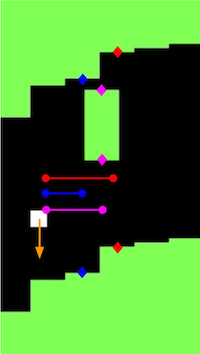
\includegraphics[width=0.3\textwidth]{pixelcopter-features}
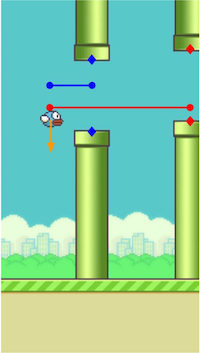
\includegraphics[width=0.3\textwidth]{flappybird-features}
\end{center}
\caption{The lines represent distances to several objects, while diamonds represent locations. The arrow represents the vertical velocity of the player.}
\label{fig:features}
\end{figure}

\subsection{Infrastructure}

The infrastructure for the game comes mostly from the PyGame Learning Environment, OpenAI gym, and keras-rl packages. 
The PyGame Learning Environment provides a nicely wrapped implementation of FlappyBird, complete with sprites and the relevant game mechanics built in. \cite{ple} \cite{openaigym} \cite{ale}
Keras-rl provides a deep reinforcement learning framework that gives us a simple interface for training agents. 
We take advantage of these two here, writing wrappers for the PLE game instance so that it is compatible with keras-rl. \cite{kerasrl}
The keras-rl package additionally provides an implementation of several algorithms that are applicable to FlappyBird, particularly Deep Q-networks and the SARSA algorithm.
For the transfer learning portion of the project, we saved weights info \texttt{hdf5} files with the Keras package.
The neural networks and much of the other deep learning architecture was also created in Keras, with a TensorFlow backend. \cite{keras} \cite{tensorflow}
This allowed us to monitor training time and other metrics inside TensorBoard.

Code for our project can be found at this link: \href{https://github.com/cdrckrgt/cs221-project} {https://github.com/cdrckrgt/cs221-project}.

\section{Model}

In this section, we describe the DQN algorithm and how it applies to our task. We use a modified version of the algorithm described in the 2013 DeepMind paper.

Again, we model the environment $\mathcal{E}$ as a Markov decision process with no knowledge of the transition probabilities or reward function at every state.
There is a set of actions that may be taken at every time-step, designated $\mathcal{A}$.
Each interaction between the agent and its environment at time $t$ produces an observation $x_t \in \mathbb{R}^{d}$ and reward $r_t$, where $d$ is the dimensionality of the environment.

As in the standard Q-learning algorithm, we consider sequences of observations, actions, and rewards $x_1, a_1, r_1, \dots, x_t, a_t, r_t$ as the state of $\mathcal{E}$ at time $t$. 
The objective of the agent is to maximize its future reward, defined as:
\begin{equation}
\displaystyle R_t = \sum_{t' = t}^{T} \gamma^{t' - t}r_{t'}
\end{equation}
such that $T$ is the termination time-step of the game.
Then the optimal Q-value function is defined as follows:
\begin{equation}
\displaystyle Q^{*}(s, a) = \max_{\pi}\mathbb{E}[R_t\ |\ s_t = s, a_t = a, \pi]
\end{equation}
such that $\pi$ is a policy that maps states to actions.
So far we have described steps to arriving at the Q-learning algorithm described by Dayans and Watkins. \cite{qlearning} 
The DQN algorithm presented by DeepMind makes numerous improvement on this algorithm by introducing a non-linear function approximator and experience replay.

\subsection{The Q-network}
Since the vanilla Q-learning algorithm does not generalize well to state spaces as large as those encountered in video games, we use a neural network to approximate the Q-value function. 
Then we have a neural network parametrized by weights $\theta$ such that $Q(s, a; \theta) \approx Q^{*}(s, a)$.
At every iteration of training $i$, we minimize the squared error between the current Q-function and the optimal Q-function, according to the loss function:
\begin{equation}
\displaystyle L_i(\theta_i) = \mathbb{E}_{s, a \sim \rho(\cdot)}[(y_i - Q(s, a; \theta_i))^2]
\end{equation}
where $y_i = \mathbb{E}_{s' \sim \mathcal{E}}[r + \gamma\max_{a'}Q(s', a'; \theta_{i - 1}\ |\ s, a]$ and $\rho(s, a)$ is a probability distribution over states and actions. 
The intuition behind this loss function is that we are minimizing the distance between our target, which is the maximum expected future reward for this state and the previous iteration's weights, and our current Q value.
We are effectively getting closer and closer to the true Q values every training iteration.
To minimize this objective function, we update the weights according to the gradient:
\begin{equation}
\displaystyle \nabla_{\theta_i}L_i(\theta_i) = \mathbb{E}_{s, a \sim \rho(\cdot)}[(r + \gamma \max_{a'}Q(s', a'; \theta_{i - 1}) - Q(s, a; \theta_i))\nabla_{\theta_i}Q(s, a; \theta_i)]
\label{eq:gd}
\end{equation}
And we've now arrived at the Deep Q-network algorithm that we can apply to our task.
It's important to note that the original DQN paper applies this algorithm to raw pixel vectors as each $x_t$, whereas we use the internal game state for each $x_t$.
This allows us to achieve the same level of performance in a much quicker fashion, since we don't need to spend the extra compute power on training a convolutional neural network to learn features for each game.
The algorithm, lifted from Mnih's paper, is described in \ref{alg:dqn}.

\begin{algorithm}
\caption{Deep Q-learning with Experience Replay}
\label{alg:dqn}
\begin{algorithmic}[1]
\State Initialize replay memory $\mathcal{D}$ to capacity $N$
\State Initialize action-value function $Q$ with random weights
\For{$\textrm{episode} = 1, M$}
    \State Initialize sequence $s_1 = \{x_1\}$ and preprocessed sequenced $\phi_1 = \phi(s_1)$
    \For{$t = 1, T$}
        \State With probability $\epsilon$ select a random action $a_t$
        \State otherwise select $a_t = \max_{a}Q^{*}(\phi(s_t), a; \theta)$
        \State Execute action $a_t$ in emulator and observe reward $r_t$ and observation $x_{t + 1}$
        \State Set $s_{t + 1} = s_t, a_t, x_{t + 1}$ and preprocess $\phi_{t + 1} = \phi(s_{t + 1})$
        \State Store transition $(\phi_t, a_t, r_t, \phi_{t + 1})$ in $\mathcal{D}$
        \State Sample random minibatch of transitions $(\phi_j, a_j, r_j, \phi_{j + 1})$
        \State Set $ \displaystyle  y_j = 
                        \begin{cases}
                            r_j & \textrm{for terminal}\ \phi_{j + 1} \\
                            r_j + \gamma\max_{a'}Q(\phi_{j + 1}, a'; \theta) & \textrm{for non-terminal}\ \phi_{j + 1} \\
                        \end{cases}
                   $
        \State Perform a gradient descent step on $(y_j - Q(\phi_j, a_j; \theta))^2$ according to equation \ref{eq:gd}
    \EndFor
\EndFor
\end{algorithmic}
\end{algorithm}

\subsection{Experience Replay}
Additionally, the algorithm presented in Mnih's paper makes use of experience replay to smooth learning and prevent divergence.
Rather than performing gradient updates on each consecutive sample, samples are stored in a ring buffer and sampled randomly during the learning phase of the algorithm. 
This has the effect of improving sample efficiency and removing the dependence of each training update on the previous training update.
Adding experience replay makes the problem conceptually similar to supervised learning, where we continuously store and update a cache of `experience' and fit our Q-function to it.

\subsection{Target Network}
Finally, we make use of a target network to further stabilize the training process. 
Note that during our gradient descent, the weights that produce our target values shift every iteration.
Instead of using these rapidly shifting weights, we copy the parameters of the training network $\theta_{training}$ to a second, identical model $\theta_{target}$.
With this identical model, we may compute the same targets, albeit with less variance by only updating the $\theta_{target}$ to match the $\theta_{training}$ with some fixed, low probability at every iteration.

\subsection{Annealed $\epsilon$-greedy Policy}
Rather than use the standard $\epsilon$-greedy policy, we opted to use a policy that annealed $\epsilon$ from some value $\alpha$ to some value $\beta$ over training.
Our goal was to incentivize exploration early on, but revert back to the usually $\epsilon$-greedy policy after some about of training.
This came from our intuition that our model would not know a great deal early on in the training, so it was most effective to explore the game's states than exploit a weak policy.


\subsection{Model Architecture}
Since we use as input to the Q-network the internal game state representation as opposed to the raw pixel inputs, we don't make use of a convolutional neural network to learn features directly from the game's pixels.
We instead make use of a multi-layered perceptron that takes as input the game's state in vector form.
In the case of FlappyBird, the state vector is a vector in $\mathbb{R}^{11}$, and contains the bird's position, velocity, and the distance, top, and bottom positions of the next two pipes.
We also added three null features to the game's state, since PixelCopter had a feature representation in $\mathbb{R}^{11}$.
PixelCopter had the same features as FlappyBird, with three additional ones: the distance to the next obstacle and the positions of the top and bottom of the obstacle.
We have three fully connected hidden layers, with dimensionality 256, 128, and 16. 
Each layer was followed by a ReLU activation, while the output layer was instead followed by a linear activation. 
This leaves us with 38,066 trainable parameters, a relatively small network compared to those that are used to learn games from pixel input.
The outputs of the Q-network for each game were the Q-values of all actions in the action space for that game.
In the case of FlappyBird, the output was two Q-values in $\mathbb{R}$, one for the action to jump, and the null action.

\section{Results}

\subsection{DQN on FlappyBird}

The DQN agent trained on FlappyBird reached superhuman levels of ability. 
The final hyperparameters are described in \ref{hyperparams-xavier}.
We see in \ref{fig:flappy-training-eps} the variance in episode reward over different random seeds for the FlappyBird game.
Each run was trained over 75,000 iterations, and we see the ability for the DQN agent to learn to play the game sometimes but fail other times.
The DQN agent performs well above the ability of the average human when it does learn to play the game, since it averages 14,177 steps before dying.
At 24 frames per second, this comes out to be 10 minutes without dying!

\begin{figure}[h!]
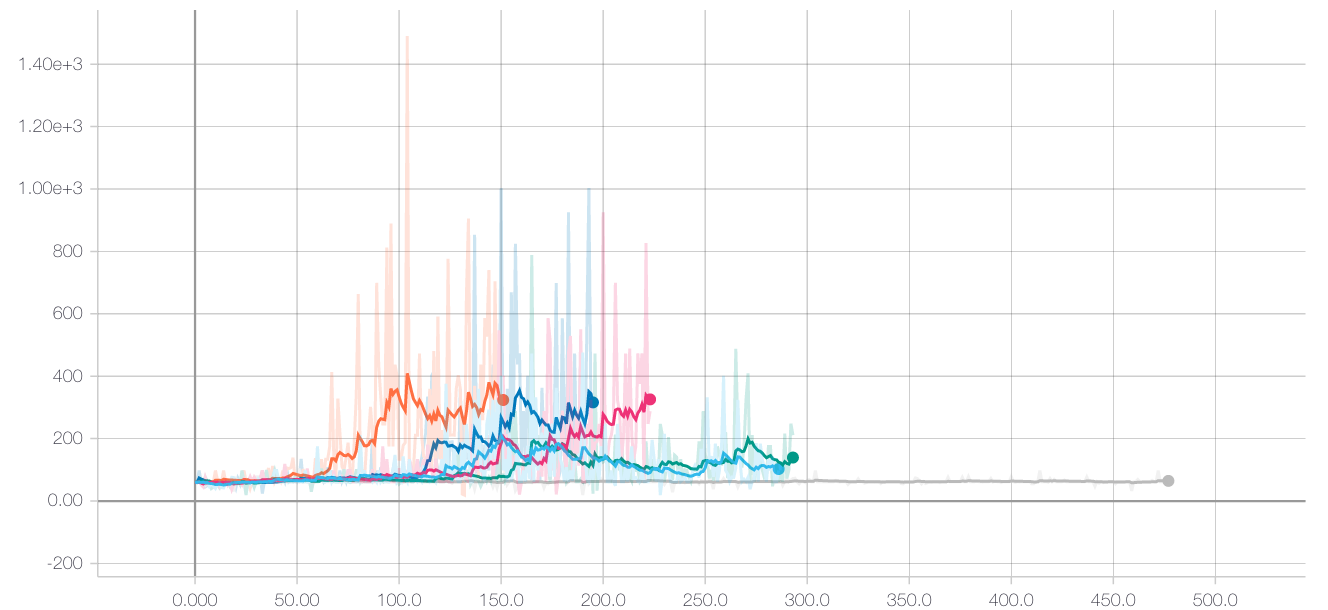
\includegraphics[width=\textwidth]{flappy-training-eps}
\caption{6 different runs for DQN on FlappyBird. The x-axis shows episode number, while the y-axis shows episode length.}
\label{fig:flappy-training-eps}
\end{figure}

\begin{table}[h!]
\centering
\begin{tabular}{ll}

\multicolumn{2}{ c }{ \textbf{Hyperparameters for Xavier-initialized networks} } \\

\\

    \begin{tabular}{| c | c |}
    \hline
    \multicolumn{2}{| c |}{FlappyBird Hyperparameters} \\ 
    \hline
    Target Model Update & 1e-2 \\
    \hline
    Learning Rate & 1e-3 \\
    \hline
    $\gamma$ & 0.99 \\
    \hline
    Annealed $\epsilon$ & 0.2 $\rightarrow$ 0.05 \\
    \hline
    Annealing Steps & 30,000 \\
    \hline
    Warm-up Steps & 100 \\
    \hline
    Memory Size Limit & 50,000 \\
    \hline
    Training Steps & 75,000 \\
    \hline
    \multicolumn{2}{| c |}{Reward Profile} \\ 
    \hline
    tick & $0.1$ \\
    \hline
    passed pipe & $1.0$ \\
    \hline
    collided & $-10.0$ \\
    \hline
    \end{tabular}

&

    \begin{tabular}{| c | c |}
    \hline
    \multicolumn{2}{| c |}{PixelCopter Hyperparameters} \\ 
    \hline
    Target Model Update & 1e-2 \\
    \hline
    Learning Rate & 4e-4 \\
    \hline
    $\gamma$ & 0.99 \\
    \hline
    Annealed $\epsilon$ & 0.2 $\rightarrow$ 0.05 \\
    \hline
    Annealing Steps & 75,000 \\
    \hline
    Warm-up Steps & 100 \\
    \hline
    Memory Size Limit & 100,000 \\
    \hline
    Training Steps & 150,000 \\
    \hline
    \multicolumn{2}{| c |}{Reward Profile} \\ 
    \hline
    tick & $0.1$ \\
    \hline
    passed pipe & $1.0$ \\
    \hline
    collided & $-10.0$ \\
    \hline
    \end{tabular}

\\
\\

\end{tabular}
\caption{These hyperparameters were obtained with lots of trial and error. If not noted here, the hyperparameter was left as the default value in Keras.}
\label{hyperparams-xavier}
\end{table}

\subsection{DQN on PixelCopter}

The DQN agent trained on the version of PixelCopter that was pulled from the source repo did not perform well.
We saw that despite trying longer training times and optimizing several hyperparameters, the agent would not learn to play the game from the feature representation that the creators shipped with the game.
The training performance for the original feature extractor on PixelCopter can be seen in \ref{fig:other-training}.
The original feature extractor did not contain information about the floor and ceiling of the environment, leading the agent to ignore the floor and ceiling and eventually crash into them.

\begin{figure}[h!]
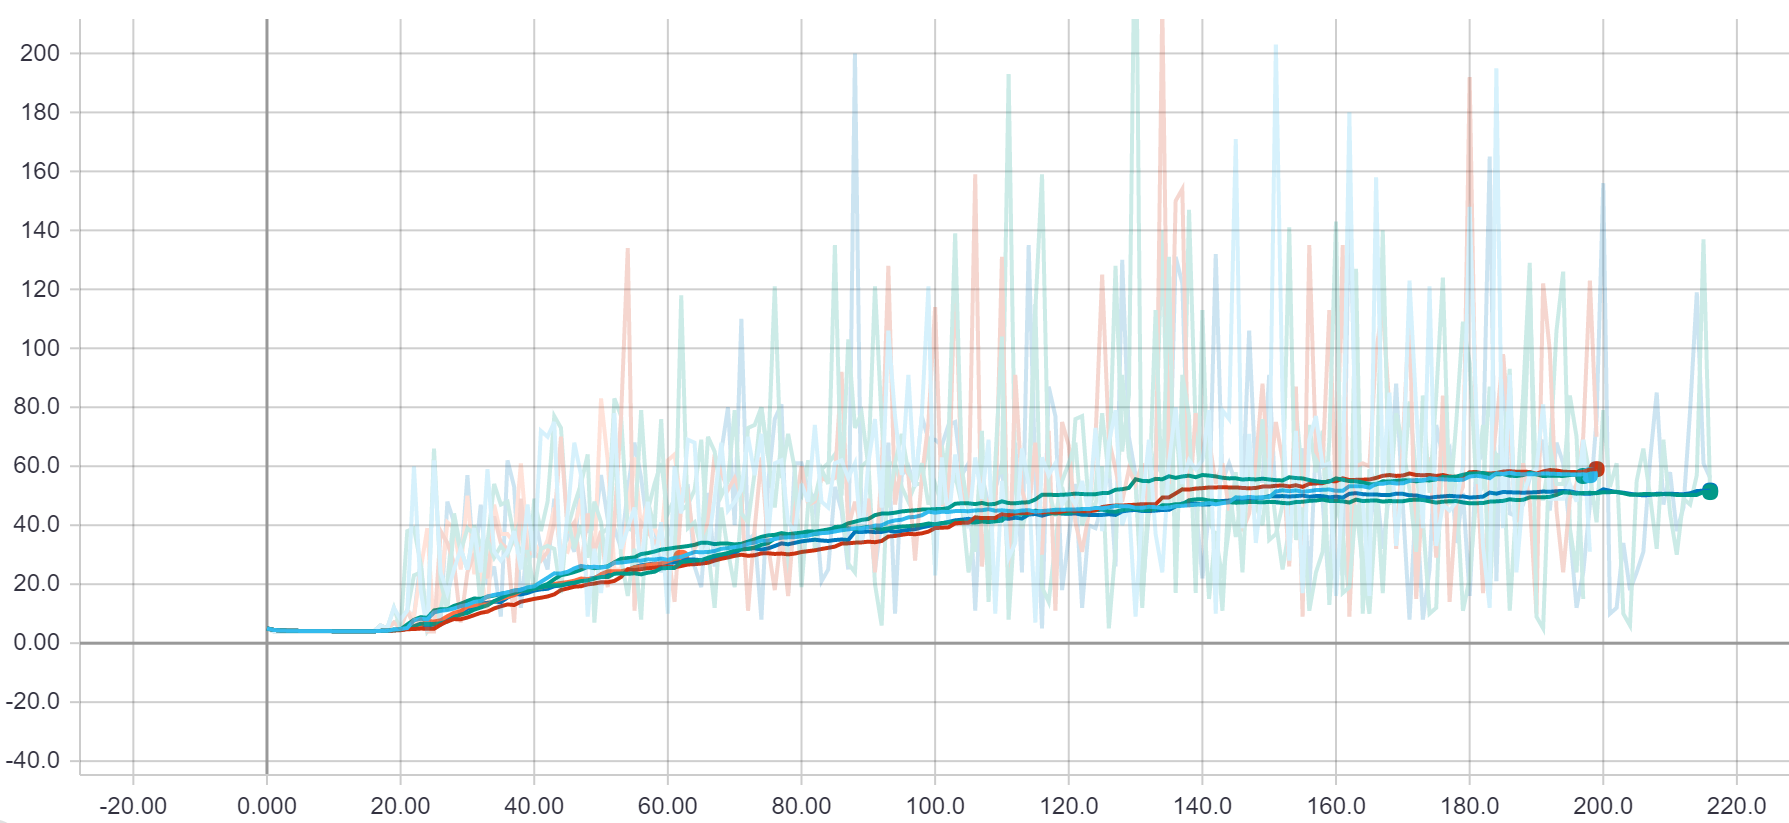
\includegraphics[width=\textwidth]{pixelcopter-training}
\caption{3 different runs for vanilla DQN on PixelCopter without optimal feature engineering. The x-axis shows episode number, while the y-axis shows episode length.}
\label{fig:other-training}
\end{figure}

We changed the features that were extracted from the game mostly for this reason, but also because we wanted the feature representations of PixelCopter and FlappyBird to be as similar as possible for the transfer learning portion of our experiments.
As seen in \ref{fig:features}, we changed the features of PixelCopter to include the positions of the next floor and ceiling pair along with the next next floor and ceiling pair.
This gave the agent the information nexessary to plan its trajectory so that it wouldn't crash into the walls.

So our updated feature extractor gave information on the floor and ceiling of the PixelCopter environment, and allowed the DQN agent to reach at least human level ability on the game. The improved training results can be seen in \ref{fig:pixelcopter-new-features}

\begin{figure}[h!]
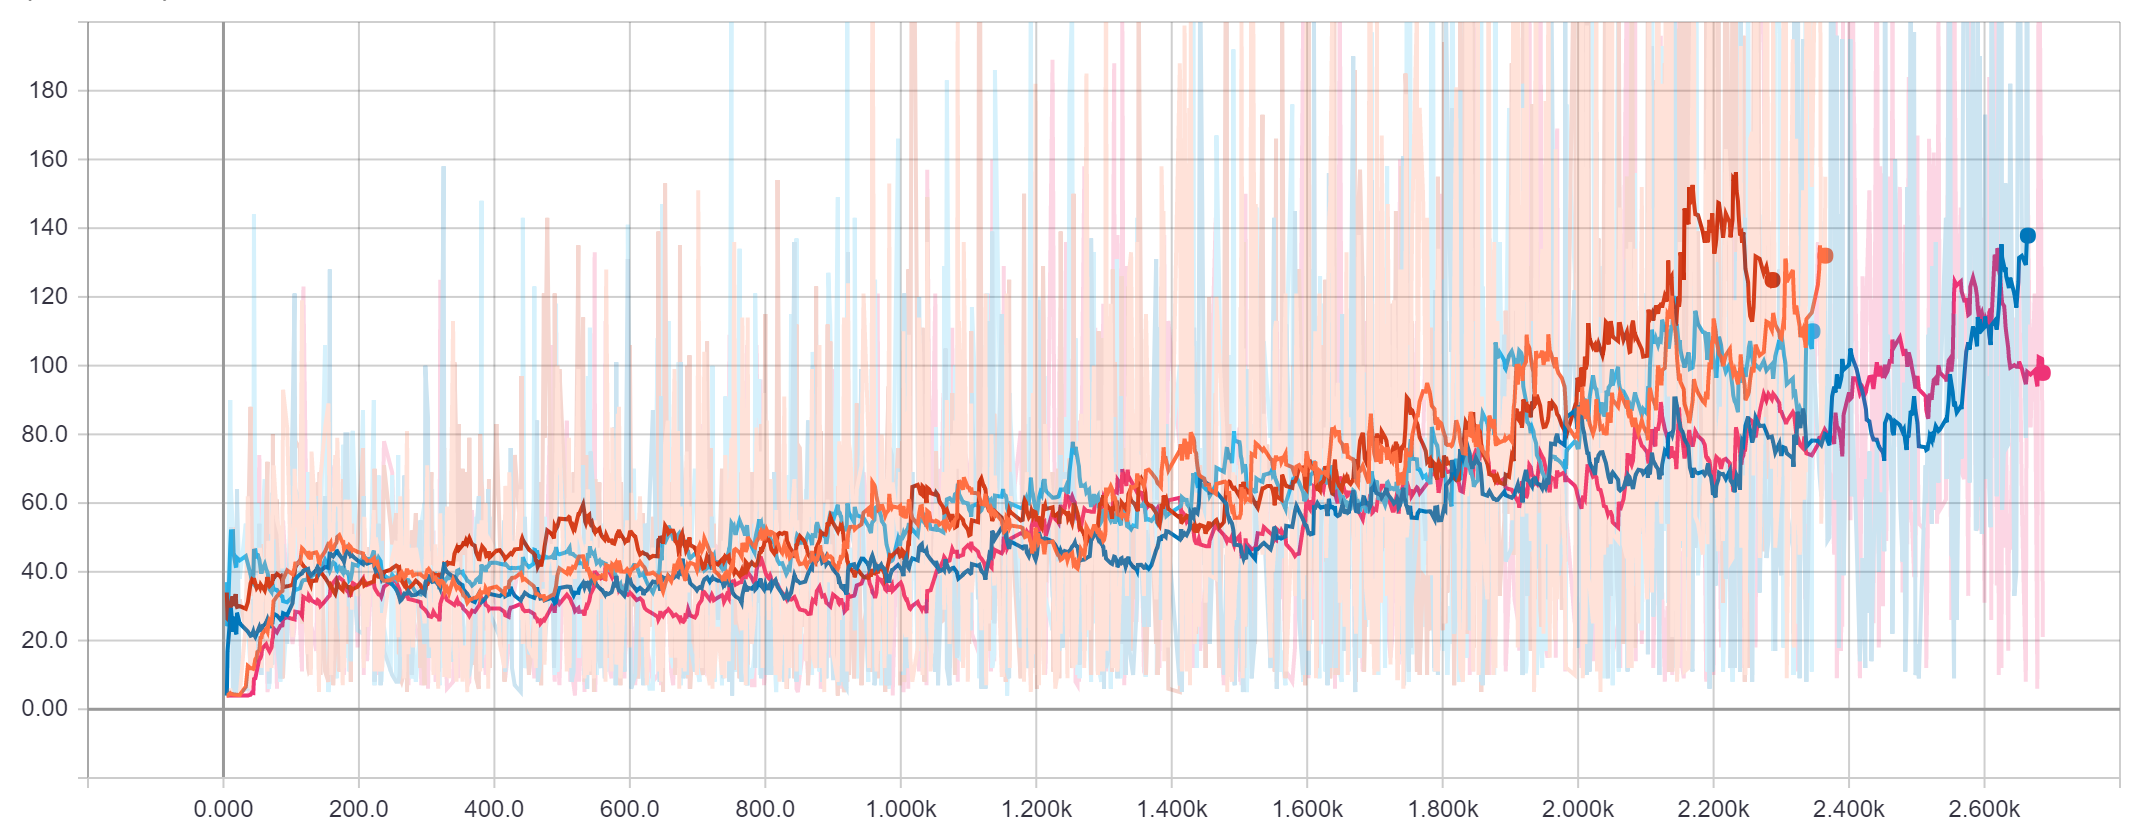
\includegraphics[width=\textwidth]{pixelcopter-new-features}
\caption{Several runs of PixelCopter training after installing a new feature extractor. The x-axis shows episode number, while the y-axis shows episode length.}
\label{fig:pixelcopter-new-features}
\end{figure}

While the training runs for both the original feature extractor and updated feature extractor look similar, the testing results showcase the superiority of our feature extractor.
The final testing results for our PixelCopter agents can be seen in \ref{fig:pixel-average-steps}.
Note that the maximum score is the average maximum score attained on each run, showing us the absolute highest that each agent can perform. 

\subsection{Transfer Learning on PixelCopter}
We implement this in a couple of different ways, with a fully trainable initialized network, and with an initialized network with frozen layers, specifically all layers but the first frozen.
There were two ways in which we tried transfer learning: simply initializing all weights with the final weights from FlappyBird, and also initializing all weights with the final weights from FlappyBird but then freezing some layers.
The latter implementation provides the effect of reducing the number of parameters needed for optimization, giving us a faster training time.
Notice in \ref{fig:transfer-training} how we don't achieve the same levels of performance as \ref{fig:pixelcopter-new-features}.

\begin{figure}[h!]
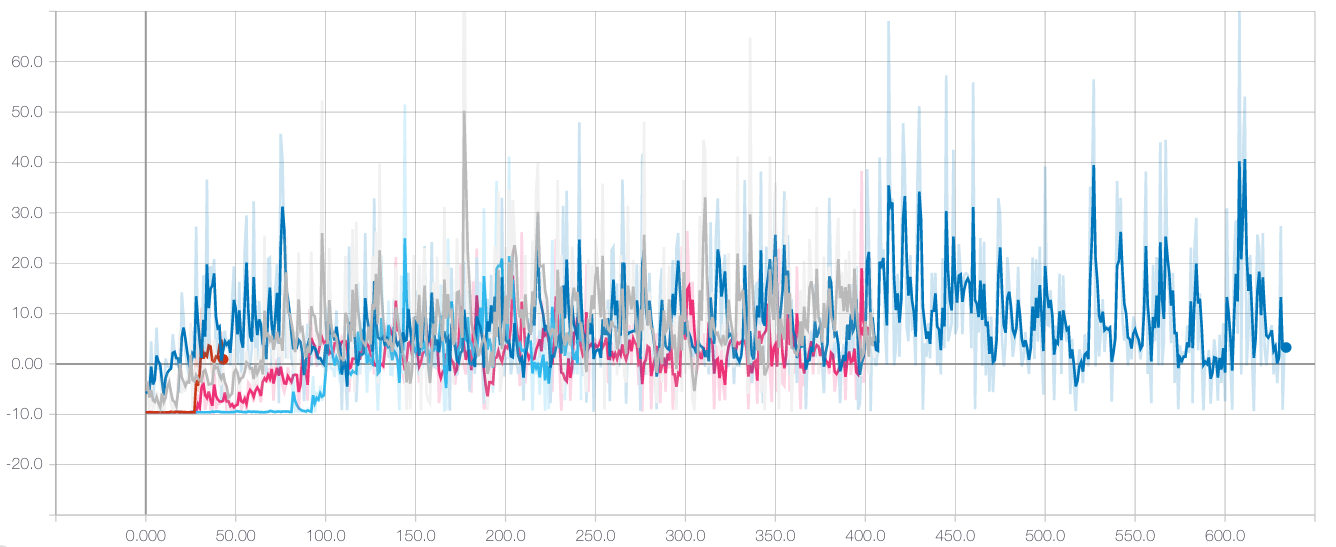
\includegraphics[width=\textwidth]{pixelcopter-transfer}
\caption{4 different runs for the DQN on PixelCopter, using weights pretrained on FlappyBird. The x-axis shows episode number, while the y-axis shows episode length.}
\label{fig:transfer-training}
\end{figure}

\begin{table}[h!]
\centering
\begin{tabular}{ll}
\\
    \begin{tabular}{| c | c | c | c | c |}
    \hline
    \multicolumn{5}{| c |}{PixelCopter Average Steps Per Episode} \\ 
    \hline
     & No TL or Feature Extractor & No TL & TL & TL with Frozen Layers \\
    \hline
    Mean & 246.47 & 373.52 & 348.58 & 148.05 \\
    \hline
    Standard Deviation & 193.91 & 377.32 & 306.87 & 116.89 \\
    \hline
    Avg. Max & 759.1 & 2552.0 & 1434.0 & 612.4 \\
    \hline
    \end{tabular}
\\
\end{tabular}
\caption{Several agents' performances on PixelCopter. Note how transfer learning with frozen layers performs markedly lower than the other agents.}
\label{fig:pixel-average-steps}
\end{table}

The final results showed how the DQN agent trained without transfer learning and with our improved feature extractor had the best performance on PixelCopter.


\section{Analysis}

\subsection{Effectiveness of Feature Engineering}
The graphs shown in \ref{fig:other-training} and \ref{fig:pixelcopter-new-features} demonstrate the effectiveness of feature engineering for PixelCopter.
With properly chosen features, we saw a vast improvement in performance, to the point where we went from effectively random movements to at least human level ability in the game.
Choosing the features wasn't a particularly difficult process -- we simply modeled the features after those found in FlappyBird, since we already knew the features that FlappyBird used and our DQN agent was able to learn FlappyBird effectively in a relatively short amount of time.
The logic behind adding the next and next next features was that the agent needed to `see' what was ahead to be able to avoid it, just like humans do!

In addition to the gains from choosing proper feature extractors, the decision to use feature extractors over raw pixel input proved to be a prudent choice. 
It is well documented that training a DQN agent from scratch with pixel inputs takes hundreds of thousands or even millions of iterations.
We saw results from our feature extracted version of DQN after only tens of thousands of iterations -- a great improvement.


\subsection{Effectiveness of Transfer Learning}
The aim of using transfer learning was to improve the average performance of DQN on PixelCopter to superhuman levels, as we did with FlappyBird.
Despite trying multiple model architectures for transfer learning, with different layers frozen vs. not frozen, we weren't able to determine that transfer learning in this specific task was effectual.
In particular, trying to freeze the hidden layers of the model was ineffective because we simply could not encode enough information on how to play the game in solely the input and output layers.
This was especially prevalent because of how we used dummy features making the FlappyBird observate space similar to the PixelCopter observation space -- since the dummy features always had values of 0 in FlappyBird, it was difficult to learn the new features in PixelCopter that weren't always 0.
Freezing transferred layers did have one tiny benefit -- the reduction in number of training parameters made training and inference slightly faster.

We theorize that the majority of the gains transfer learning has shown on reinforcement learning tasks in gameplay have come from the convolutional neural network not having to be trained from scratch, and less so from the fully connected layers that follow.
Because we opted for feature engineering over a CNN, we lost out on the performance gain that would have resulted from transfer learning.
The relatively small size of the neural net that approximated the Q-function didn't benefit very much in terms of training speed, even when the state spaces of the game were made to be as similar as possible.

\subsection{Expansion to Pixel Inputs}
The vanilla DQN model trained on PixelCopter did not generally perform well, even with much longer training times and hyperparameter tuning. Our hypothesis is that the state vector that the game produces doesn't yield enough information about the game for the model to learn how to play. Only the wall directly above and below the Pixelcopter is shown to the model, leaving the rest of the terrain unknown until the PixelCopter flies past it. One way to approach this issue is to simply feed the pixel representation of the game's state as image input to the model, which would necessitate the use of CNNs. We don't know the effectiveness of transfer learning on solely fully-connected layers, and hopefully this goes to show us that we might want to continue with CNNs and learning from pixel input in the future.

Because of what was discussed on the effectiveness of transfer learning, many times throughout the project we considered moving towards pixel input. 
The result would be more impressive -- not having to encode information about the game would make this end-to-end reinforcement learning task much cleaner and robust.
We opted not to do this early on because we had little experience with convolutional neural networks and image tasks.
This, combined with our desire to iterate quickly over model architectures, hyperparameters, etc. pushed us to use feature engineering over convolutional neural networks. 

Now that we know the ineffectiveness of transfer learning on solely fully connected layers, we would have definitely chosen to use pixels as input.

\section{Conclusion and Future Work}
Deep reinforcement learning has proved to be an excellent player of FlappyBird and PixelCopter, considering that with both games on the vanilla DQN agents, we could not beat the trained agent.
Our hopes of transfer learning speeding up training time and improving absolute performance were not met, and we determined that transfer learning didn't have a significant impact on the training process.

In the future, we'd extend our experiment to compare our feature extractors performance to that of a convolutional neural network. 
We think that our methodology applied to CNNs would have led to a much more successful experiment. 
In addition to this, we hope to apply reinforcement learning to games with higher complexity, much like what OpenAI has done with Dota and DeepMind has done with Go.
On an even wider scale, we foresee that many computationally difficult optimization problems can be cast to reinforcement learning problems, where we might achieve decent approximate solutions in smaller timeframes than conventional techniques.
This could impact a wide array of peoples, industries, and technologies around the world, so we think it's an exciting thing to study!

\bibliography{ref}
\bibliographystyle{plain}


\end{document}

